\chapter{蓝屏与解决蓝屏}
\label{cha:recover-from-bsod}

\begin{intro}
  这一章,我们将介绍令大多数人都头痛的问题——蓝屏死机,以及解决蓝屏问题的方法。读完本章,你应该可以找到下面这些问题的答案:
  
  \begin{itemize}
    \item 为什么我的电脑会蓝屏?
    \item 为什么我现在看到的蓝屏和以前的好像不一样?
    \item 蓝屏画面上的东西是什么,有什么用?
    \item 我怎么才能解决电脑的蓝屏问题?
  \end{itemize}
\end{intro}

我们在日常使用电脑的过程中,总不可能避免遇到各种各样的问题,其中最为出名的要数「蓝屏死机」了。蓝屏令人恼火,但更多的却是无可奈何,因为大多数人只能盯着那蓝蓝的界面,等着电脑自动重启,然后继续使用,祈祷着不会再一次出现同样的问题。但我们真的束手无策吗?在此,不妨来详细了解一下这蓝屏,顺便尝试着手清除它的隐患。

认识蓝屏,先来看看它是如何起源与发展的吧。

\section{:(}

\begin{figure}[htb!]
  \centering
  
\includegraphics[width=.65\textwidth]{assets/advanced/Win-10-BSoD.png}
  \caption{Windows 10 与 11 的蓝屏界面}
  \label{fig:Win-11-BSoD}
\end{figure}

蓝屏死机,英文叫 BSoD(Blue Screen of Death,「死亡蓝屏」,很形象啊)。如今的 2024 年,大多数个人电脑上搭载的都是 Windows 10 或 Windows 11 操作系统,它们的蓝屏错误界面很有特色,大概如\autoref{fig:Win-11-BSoD}。

以一个大大的文字表情「 :( 」开头,代表了人们遇到这个界面时的心声,接下来是一些说明性文字,看起来很简洁。略览这些文字,我们不难推测,\regcolor{蓝屏死机说明操作系统遇到某种极为严重的错误,被迫终止运行}。但最初的蓝色错误界面(事实上是如今蓝屏错误的前身)与这可有天壤之别。

\subsection{DOS 时代}

第一个名叫「Windows」的操作系统是微软在 1985 年 11 月发布的 Windows 1.0,它是一个基于 DOS(Disk Operating System,磁盘操作系统)的操作系统——也就是说,这时的 Windows 与其说是「操作系统」,不如说是在 DOS 这个真·操作系统上运行的一款大型软件。它的第一个版本 Windows 1.01 有着神奇的缺陷——只能在特定 DOS 版本下运行,高了就出错。这一错,造就了历史上最早的「蓝色错误界面」。至于为什么是蓝色的……谁让 Windows 1.0 的启动界面就是蓝底白字呢:

\begin{figure}[htb!]
  \centering
  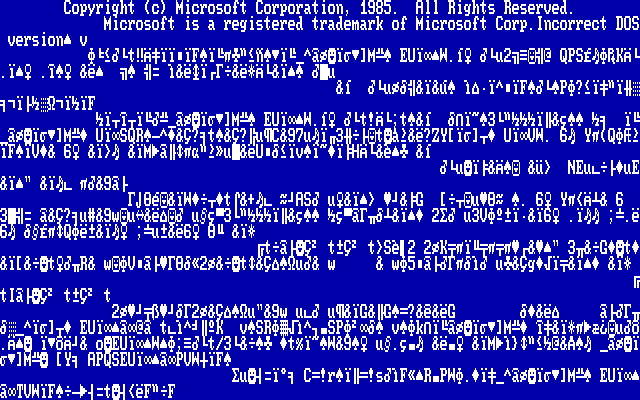
\includegraphics[width=.7\textwidth]{assets/advanced/Win-1.0-Error.png}
  \caption{Windows 1.0 的错误界面}
  \label{fig:Win-1.0-Error}
\end{figure}

在这个错误界面最上方,可见一些微软的版权信息,紧接着就是一句「不正确的 DOS 版本」昭示错误,随后便是满屏的乱码。这是由于那时的电脑,没有独立的显存,而是用内存的一块区域当作显存。错误的 DOS 版本导致 Windows 徽标那张图所在内存出错,又因为当时的 Windows 缺乏内存保护,于是溢出到显存区域,在屏幕上显示出乱七八糟的内容。之后的 Windows 1.02 版本似乎修复了这个问题,但 Windows 2.03 版本也有同样的 bug,呈现形式也是这样\CJKsout*{,所以微软你到底是修了还是没修呢}。

1990 年,微软发布了 Windows 3.0 操作系统,这个版本获得了巨大成功,发布的半年内就卖了 200 万份。它仍然基于 DOS,但带来了更好的性能……与更新的报错界面。值得注意的一点是,在这个版本的 Windows 中,用户可以按下 \keys{Ctrl + Alt + Delete} 来手动触发错误\CJKsout*{(随时随地蓝屏)}。之后发布于 1994 年的 Windows 3.2 则是第一个得到广泛使用的中文版 Windows 系统(还可以玩扫雷哦),于是我们可以看到\autoref{fig:Win-3.2-Error} 这样带中文的蓝色错误界面。

\begin{figure}[htb!]
  \centering
  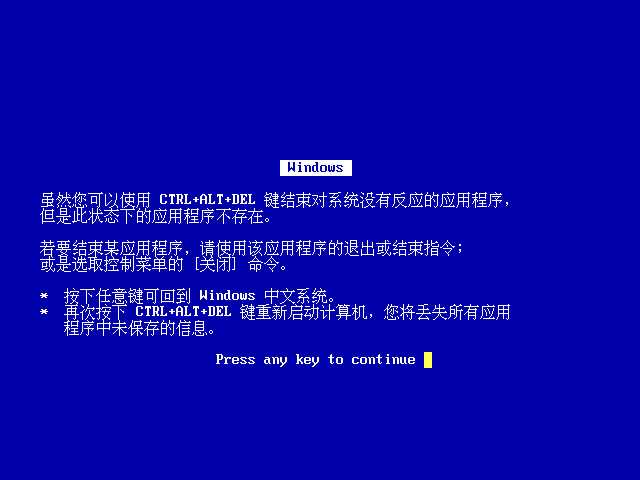
\includegraphics[width=.62\textwidth]{assets/advanced/Win-3.2-Error.png}
  \caption{Windows 3.2 的中文错误界面}
  \label{fig:Win-3.2-Error}
\end{figure}

不过仍然与之前一样,这错误界面的原因并不是系统崩溃:真正崩溃的话,计算机早就退回那黑黑的 DOS 界面了,不会提供回到 Windows 的机会。但与之前不同的是,这个错误界面会提示用户系统出错的原因,更有了现代蓝屏的味道。

次年,微软又发布了新一代 Windows,这次微软开始以两位数年份命名产品,叫作 Windows 95(著名的 IE 浏览器就是在这个系统中首次亮相的)。三年后,微软又发布了 Windows 98;到了 2000 年,微软\CJKsout*{发现把新系统命名为 00 不太合适,}将新发布的系统命名为 Windows Me,这个「Me」不是英文的「我」,而是代表「千禧年版(Millennium Edition)」。这三个系统后来统一被大家称呼为「Windows 9x」(虽说最后一个似乎不太一样),想必它们的蓝屏界面也差不多。

\begin{figure}[htb!]
  \centering
  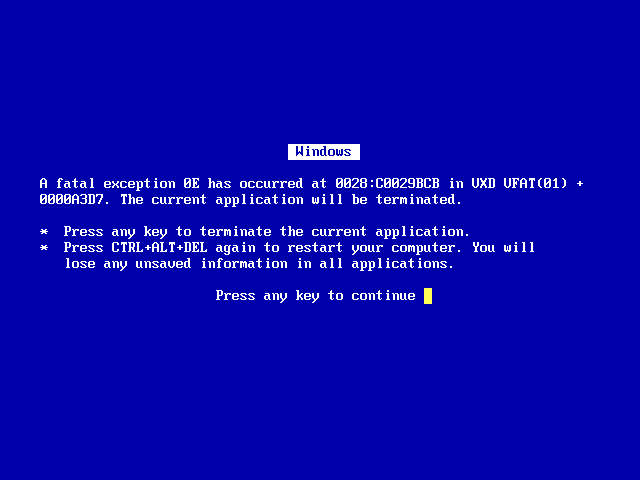
\includegraphics[width=.62\textwidth]{assets/advanced/Win-95-Error.png}
  \caption{Windows 95 的错误界面}
  \label{fig:Win-95-Error}
\end{figure}

嗯……看来不仅是 Windows 9x 之间差不多,它们与 Windows 3.x 也差不多,但与之前的相比增加了错误代码与错误发生的内存地址,帮助用户排查错误。然而,即便是中文版的 Windows 9x,蓝屏界面语言也依然是英文,微软似乎去掉了蓝屏界面的本地化。\CJKsout*{(开倒车?)}

无论是 1985 年的 Windows 1.0,还是 2000 年的 Windows Me,它们的底层都是 DOS。然而,随着计算机硬件的快速发展,DOS 的底层架构渐渐落后于时代。到 Windows Me 发布时,基于 DOS 的 Windows 已经走向衰落。两年后,Windows XP 横空出世,更标志着微软将重心全面脱离 DOS。此后,基于 DOS 的 Windows 系统一个接一个走向了时间的坟墓里,湮没在历史的沙海下。而名为「NT」的技术接过大旗,推动 Windows 继续向前发展。

\subsection{早期 NT 时代}

自 1985 年起的几年,微软除了开发自家的 Windows 之外,还在与美国科技公司 IBM 合作开发一款名叫「OS/2」的操作系统,这个系统不是很出名,毕竟它的目标是 IBM 自家的计算机。到了 1988 年 11 月,微软的一个开发团队准备改进当时的 OS/2,使之成为一个兼容 POSIX(可移植操作系统接口)的多用户操作系统,起名「NT OS/2」\footnote{那时 NT 代表「New Technology」,但后来却失去了含义,变成了单纯的代号。}。

\begin{note}
  有关 IBM 这段开发个人计算机的历史,在超越篇的\chapref{cha:program-and-arch}一章中你还会看到。
\end{note}

之前提到过,Windows 3.0 非常畅销,于是\CJKsout*{微软飘了},开发团队开始用 Win32 接口代替 OS/2 的那些接口。这 Win32 是现有的那些基于 DOS 的 Windows API 的 32 位扩展版,使得现有的 Windows 程序能很轻松地移植到 NT 平台。微软觉得很棒,但 IBM 很不爽,随后在 1990 年终止了与微软的合作,微软开发的东西也变成了「Windows NT」,而这也是现今 Windows 系统的内核。

不同于那些基于 DOS 的 Windows,Windows NT 采用自己的底层,直接运行在电脑硬件上。Windows NT 的第一个大版本系列是 Windows NT 3.x(不是刚刚介绍过的 Windows 3.x 哦),包括 1993 年发布的 3.1、1994 年发布的 3.4 与 1995 年发布的 3.51。从这个系列起,Windows 蓝屏可以真正地叫做蓝屏了,因为它来自整个系统运行时的崩溃,一崩溃就只能重启。

\begin{figure}[htb!]
  \centering
  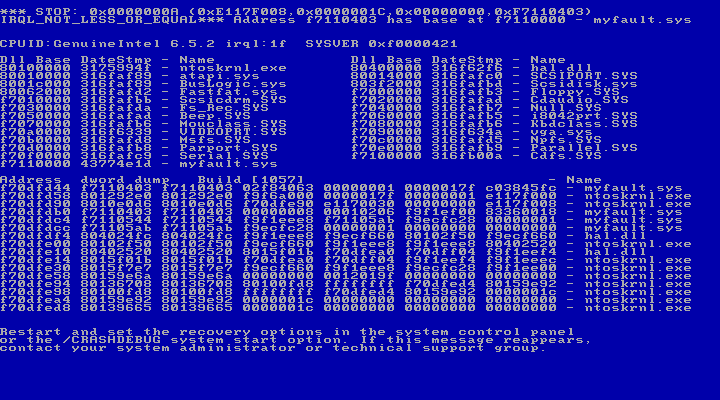
\includegraphics[width=.62\textwidth]{assets/advanced/Win-NT-3.51-BSoD.png}
  \caption{Windows NT 3.51 的蓝屏界面}
  \label{fig:Win-NT-3.51-BSoD}
\end{figure}

这是一张 Windows NT 3.51 的蓝屏截图,可以看到上面包含了许多复杂的信息,大概分为四个部分:
\begin{itemize}
  \item 第一行是由一个十六进制数代表的蓝屏错误代码(指示错误类型)、四个十六进制数代表的错误参数,第二行是错误的名称以及发生的内存地址;
  \item 接下来一大段展示电脑刚才已经加载的各种驱动;
  \item 第三部分则是出错时的内存堆栈状况;
  \item 第四部分则告诉用户一些建议的操作,例如重启、设置恢复选项、寻求帮助什么的。
\end{itemize}

1996年,Windows NT 4.0 发布。这个系统看起来与 Windows NT 3.x 大同小异,当然蓝屏界面与 Windows NT 3.x 也几乎一致,没什么好看的。

这样的蓝屏虽然看起来很吓人,满屏幕密密麻麻看不懂的东西,却方便了用户在后续寻求帮助时,让专业人士来分析问题,因为它包含了排查错误所需的许多信息。不过有些时候蓝屏显示的信息不是很多,或许是这时的错误没有那么多信息来给系统显示。

2000 年,微软发布了 Windows 2000 操作系统(又称 Windows 2K),即便它属于 NT 系列,却使用了与此前 DOS 系列类似的「年份命名法」,或许在千禧年发布的东西总要沾点它的光呢。在这个系统中,微软将曾经 Windows 95 与 98 里的许多特性都引入进来,让 NT 系列成为开发的主赛道。不过 Windows 2000 的蓝屏界面没有之前 NT 系列那么眼花缭乱,东西比较少,但这之中基本的东西,诸如蓝屏代码、参数,内存地址,蓝屏转储,建议话语之类还是有的,像这样:

\begin{figure}[htb!]
  \centering
  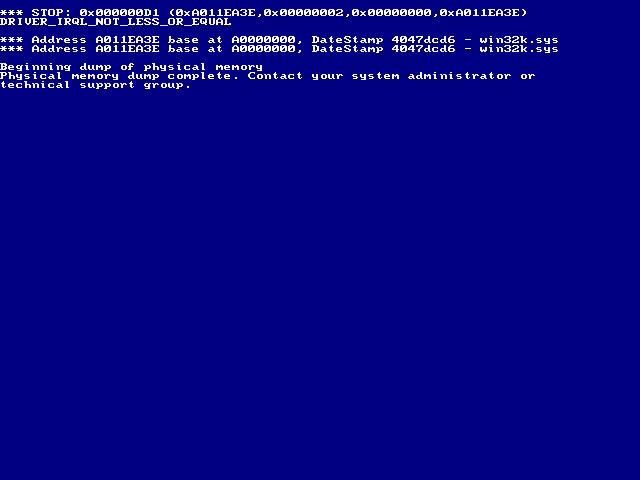
\includegraphics[width=.7\textwidth]{assets/advanced/Win-2K-BSoD.png}
  \caption{Windows 2000 的蓝屏界面}
  \label{fig:Win-2K-BSoD}
\end{figure}

Windows 2000 的后继者便是大名鼎鼎的 Windows XP,在前者发布的次年便很快发布,名字中的「XP」代表「e\underline{xp}erience」(体验)。正如其名,Windows XP 为用户带来了不同于以往 NT 系列的体验,包括令人耳目一新的用户界面与大量性能改进。这个系统实在过于经典,以至于大概二十年后的现在,仍有一些重要设备在运行它。

Windows XP 的蓝屏界面长这样:

\begin{figure}[htb!]
  \centering
  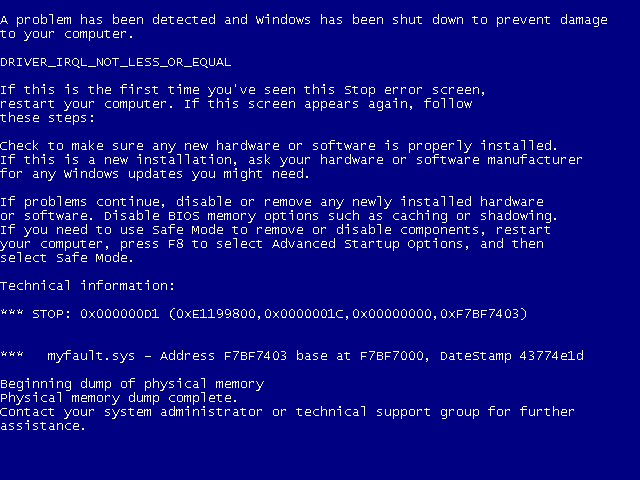
\includegraphics[width=.7\textwidth]{assets/advanced/Win-XP-BSoD.png}
  \caption{Windows XP 的蓝屏界面}
  \label{fig:Win-XP-BSoD}
\end{figure}

可以看到蓝屏界面的开头多了一句话:

\begin{quoting}
  A problem has been detected and Windows has been shut down to prevent damage to your computer.
\end{quoting}

什么意思呢?

\begin{quoting}
  检测到了一个问题,Windows 已停止运行从而避免损害您的电脑。
\end{quoting}

\CJKsout*{多贴心啊!}这比以前直接一个「STOP」糊脸似乎温和得多,但仍然改变不了它是个蓝屏界面的事实。不过接下来的大段文字,几乎都是在向用户提供建议,例如重启、检查安装的新硬件及其驱动等等,不得不说确实「人性化」许多。当然,放在最后的还是必不可少的蓝屏代码、错误参数以及进程信息。

Windows XP 的后继者是 Windows Vista,它于 2007 年正式发布,但似乎是一个名不见经传的系统。确实,比起它的前任与后继者,它似乎逊色许多。它的后继者是同样大名鼎鼎的 Windows 7。看起来微软的命名是自由的,我们没法知道这个「7」为什么是「7」,只需要知道它是「7」就好了。Windows 7 于 2009 年发布,带来了好看的界面与至今津津乐道的体验。不过从 Windows XP 到 7,蓝屏界面一直没有发生变化,而下一次的变化,就大到要进入下个时代了。

\subsection{「简洁」时代}

在 2010 年左右的这段时间,微软想进军移动市场,顺便来一个移动桌面平台「大一统」(虽然目前来看,结果不怎么样,参见\chapref{cha:software-installation})。在此理念影响下,微软在 2012 年发布的 Windows 8 更像是一个平板电脑操作系统,操作逻辑与之前的 Windows 相去甚远,甚至连开始按钮都惨遭舍弃。用户当然不买账:「跟了我们这么久的开始按钮怎么能说丢就丢呢?」于是微软在随后的 Windows 8.1 把开始按钮加了回来,但也仅此而已,未能改变它「看起来像给平板用的系统」的本质,愿意用 Windows 8 系列的用户也还是不多。

至于蓝屏界面,自 Windows 8 开始,它就从曾经的类似命令行上一大堆信息的画面变成了现在标志性的「 :( 」画面,处处透露着一股「简洁」之风。

\begin{figure}[htb!]
  \centering
  
\includegraphics[width=.6\textwidth]{assets/advanced/Win-8.1-BSoD.png}
  \caption{Windows 8.1 的蓝屏界面}
  \label{fig:Win-8.1-BSoD}
\end{figure}

啊,时隔多年,我们再一次在蓝屏界面上看到了中文,真是可喜可贺、可歌可泣啊。但这提供的信息量相比之前的 Windows XP 到 7 的蓝屏界面少了许多,这里只告诉你「你的电脑有问题,得重启」,反倒没有了之前所看到的那一大段具体建议。此外,蓝屏代码由之前的十六进制数字变成了一串英文\footnote{事实上早期 NT 时代中也出现过这些英文,不过它们并没有「蓝屏代码」的地位。而「简洁」时代的蓝屏代码也不全是英文,偶尔会有数字出现。}。比起之前那不明所以的数字,这样的错误代码倒是显得更直观,但还是很笼统。至于技术层面的错误信息,除了这个蓝屏代码就没有其他的了,甚至没有与之相关的进程信息,这导致普通用户只能根据这个蓝屏代码来搜索解决方案,增大了排查难度。\CJKsout*{(看来微软这倒车是越开越远了啊。)}

Windows 8.1 的下一代是 2014 年发布的 Windows 10 \CJKsout*{(9 呢?记住,微软是自由的。)},是如今广泛使用的操作系统。这次微软倒是长记性了,把开始菜单弄回来了,不过变成了「磁贴式」,倒也方便许多。Windows 10 的蓝屏界面在本节开头已经看到过了,与上一代不同的地方在于:它多了一个指向其旁边\href{https://www.windows.com/stopcode}{蓝屏错误疑难解答}链接的二维码,似乎能帮助用户解决问题。(但真的有用吗?请看后文。)

Windows 10 的下一代是 2021 年发布的 Windows 11,正式版的蓝屏界面与 Windows 10 的一模一样,但值得一提的是,在某个时段的预览版中,蓝屏界面变成了黑色,就像这样:

\begin{figure}[htb!]
  \centering
  
\includegraphics[width=.6\textwidth]{assets/advanced/Win-11-Pre-BSoD.png}
  \caption{Windows 11 早期预览版的蓝屏界面}
  \label{fig:Win-11-Pre-BSoD}
\end{figure}

嗯……怎么说呢,看起来死气沉沉的。

到这里,我们就把所有 Windows 系统不同的蓝屏全看了一遍。蓝屏作为一个系统崩溃错误界面,承担的职责应当是显示错误信息,便于用户或技术人员排查。不难发现,早期的蓝屏虽然不太好看,但尽到了自己的职责,但如今的蓝屏更多的是发扬「简洁即美」的思想,却似乎把自己的职责抛开不顾了……不愧是你,微软。

\section{搞定蓝屏}

\subsection{什么是「内存转储」}

如今 Windows 10/11 的蓝屏界面只提供了错误代码,如果你尝试过去网上搜索它,一般得到的都是非常笼统的说辞,诸如「使用安全模式启动」「尝试更新驱动」「尝试检查磁盘错误」「尝试系统还原」甚至「尝试重装系统」。这也难怪,毕竟蓝屏代码就那么几个,但引起蓝屏的因素却如同恒河沙数,自然只能把想到的全试一遍。虽说重装系统能解决 99\% 的问题\footnote{\CJKsout*{顺带一提,重买可以解决 100\% 的问题。}},但不建议如此大动干戈,毕竟数据无价。而事实上其他方案都是「碰运气」,能搞定算我们运气好。我们真正需要的,是对症下药——找出问题的根源,着手消除它。

你如果仔细观察过之前「早期 NT 时代」的各种蓝屏界面的话,可能会发现最后一段有一句话:

\begin{quoting}
  Beginning dump of physical memory.
\end{quoting}

这就要说到 Windows 会在蓝屏时做些什么「幕后工作」了。在蓝屏发生之时,系统会收集发生错误的进程所在的内存与堆栈内容,并将它们放入一个「蓝屏内存转储文件」中。如今的蓝屏上「我们只收集某些错误信息」说的就是这个事。也就是说,即便蓝屏界面上没有了相关的技术信息,我们也可以通过分析内存转储文件的方式查找真正的蓝屏原因。当你遇到蓝屏时,不妨在重启后立刻打开 \MissingVerb{C:\Windows\Minidump} 目录(如果系统提示【你当前无权访问该文件夹】,请点击【继续】),你应当能看见一个(或多个)\MissingVerb{dmp} 格式的文件。它们就是之前遇到蓝屏时,系统留下的转储文件。

\begin{figure}[htb!]
  \centering
  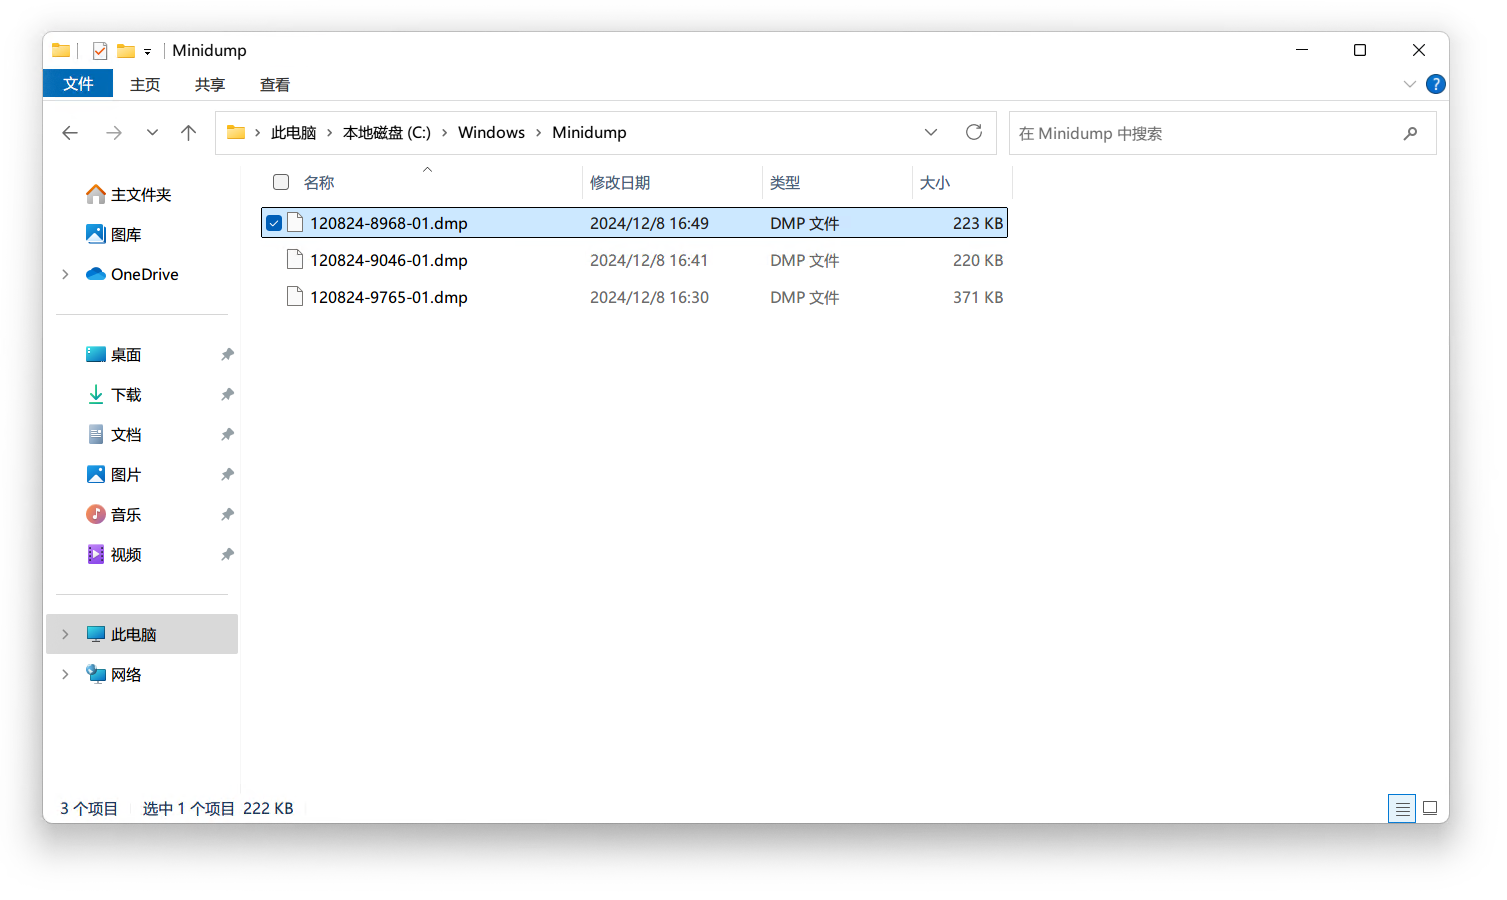
\includegraphics[width=.75\textwidth]{assets/advanced/Dump_files.png}
  \caption{电脑里的蓝屏内存转储文件}
  \label{fig:Dump_files}
\end{figure}

根据文件的修改日期,我们可以找到历次蓝屏所对应的转储文件。将它们复制出来(如果系统仍然不稳定,可以尽快复制到其他电脑上),我们就可以对它们进行分析,从而找出具体的蓝屏原因了。

\begin{note}
  如果在遇到蓝屏后,\MissingVerb{C:\Windows\Minidump} 下没有产生转储文件,则需要按后文的方法修改系统转储设置。
\end{note}

\subsection{分析转储文件}

要分析这些内存转储文件,我们需要特殊的工具——WinDbg(Windows 调试器)。

打开 Microsoft Store,也就是微软应用商店,在上面搜索「WinDbg」,跳出来的第一个应用就会是它,点击【获取】,等待一会,就安装好了。如果不想在 Microsoft Store 安装,也可以去微软提供的 WinDbg 官方页面(\url{https://learn.microsoft.com/zh-cn/windows-hardware/drivers/debugger/})下载。

\begin{figure}[htb!]
  \centering
  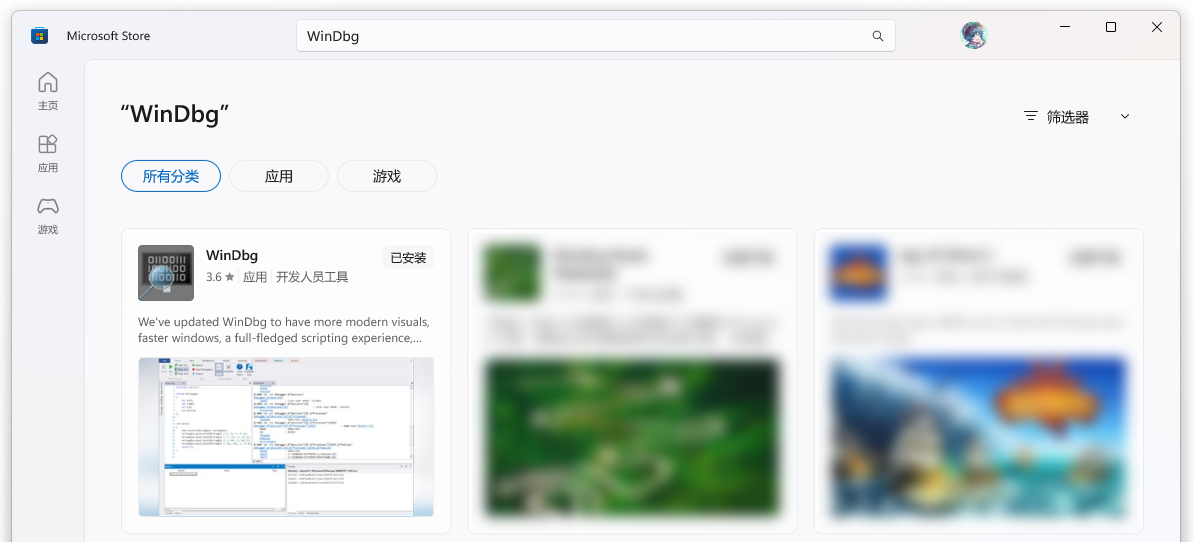
\includegraphics[width=.8\textwidth]{assets/advanced/WinDbg.png}
  \caption{在微软商店搜索 WinDbg}
  \label{fig:WinDbg}
\end{figure}

安装好之后,电脑上的蓝屏内存转储文件就能直接双击打开了。转到之前设置转储选项时看到的内存转储路径中,打开最近一次蓝屏的转储文件,你大概会看到这样的界面:

\begin{figure}[htb!]
  \centering
  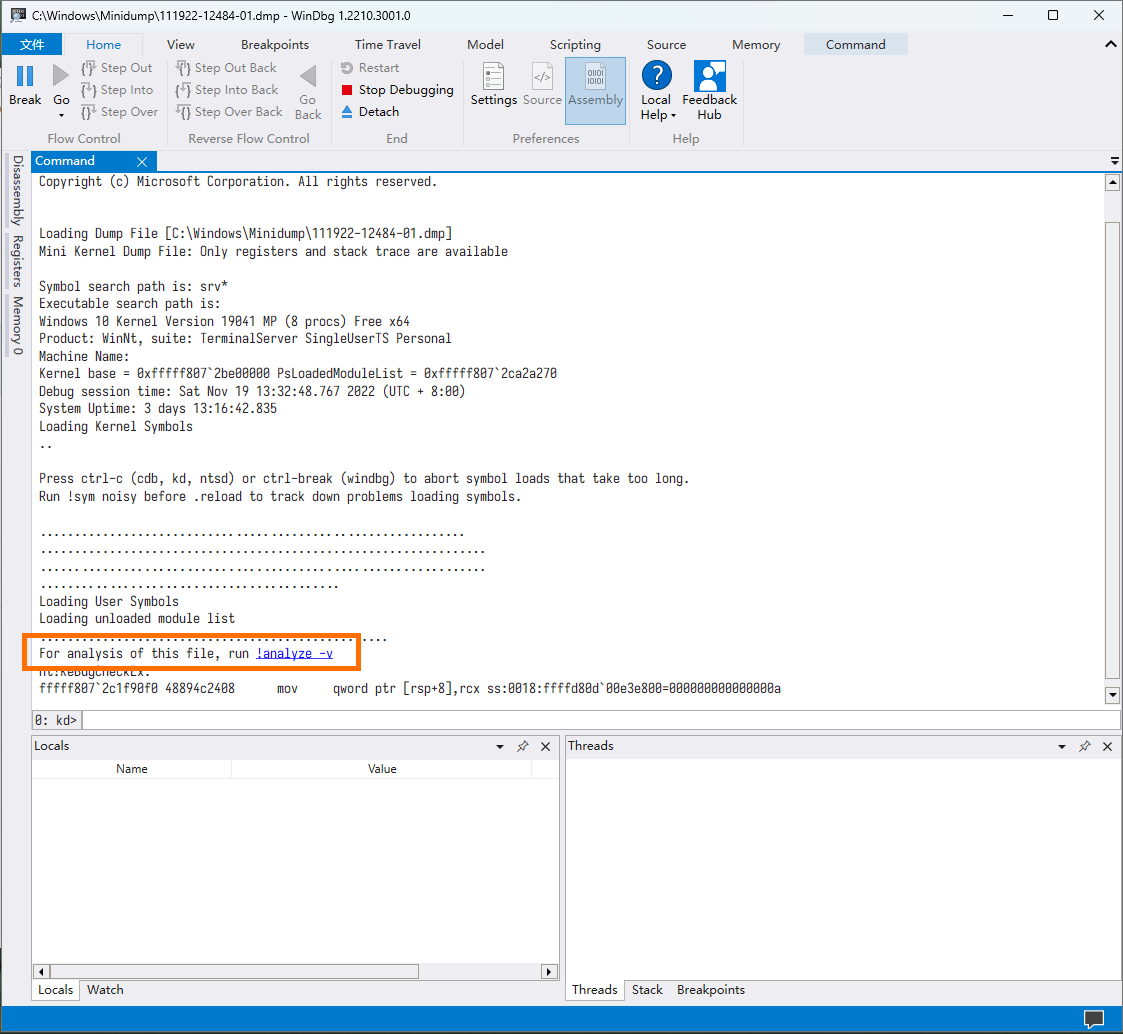
\includegraphics[width=.8\textwidth]{assets/advanced/WinDbg-1.png}
  \caption{用 WinDbg 加载蓝屏转储文件}
  \label{fig:WinDbg-1}
\end{figure}

其中偏下方的位置有用醒目的蓝色写出的 \MissingVerb{!analyze -v},结合它旁边的说明就能知道,\regcolor{运行这个命令就可以分析转储文件}。WinDbg 也很方便,\regcolor{点击这里的蓝色文字就可以运行命令}。在命令执行过程中,左侧中下部的状态会显示 \MissingVerb{*BUSY*},同时最下方会显示正在从服务器下载哪些所需的文件。这时可以喝杯茶,等待分析过程完成。

\begin{figure}[htb!]
  \centering
  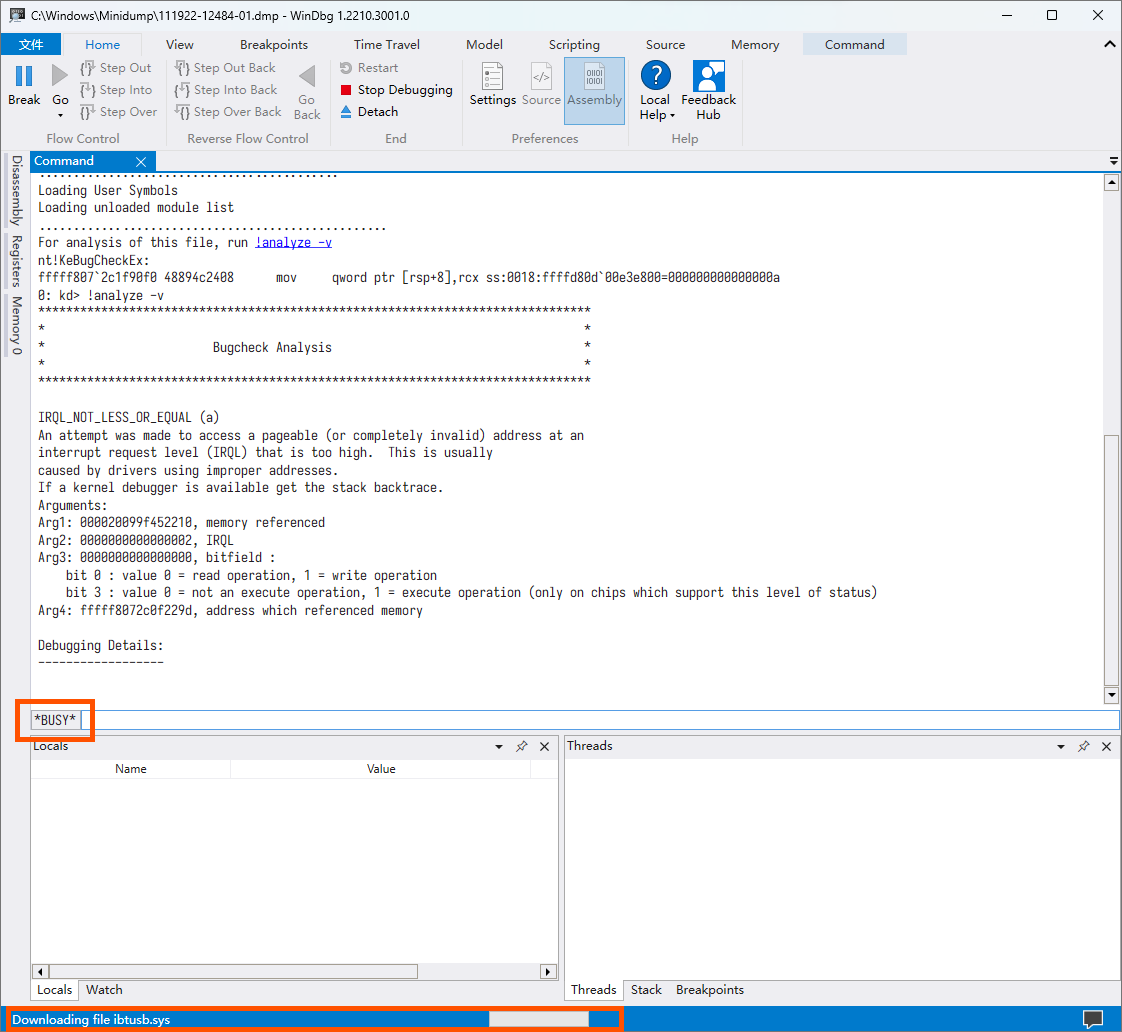
\includegraphics[width=.75\textwidth]{assets/advanced/WinDbg-2.png}
  \caption{启动 WinDbg 的分析命令}
  \label{fig:WinDbg-2}
\end{figure}

分析完毕之后,你会发现出来了一大堆令人眼花缭乱头晕目眩的分析结果,这些结果都是以灰色背景显示的,如\autoref{fig:WinDbg-3} 所示。

\begin{figure}[htb!]
  \centering
  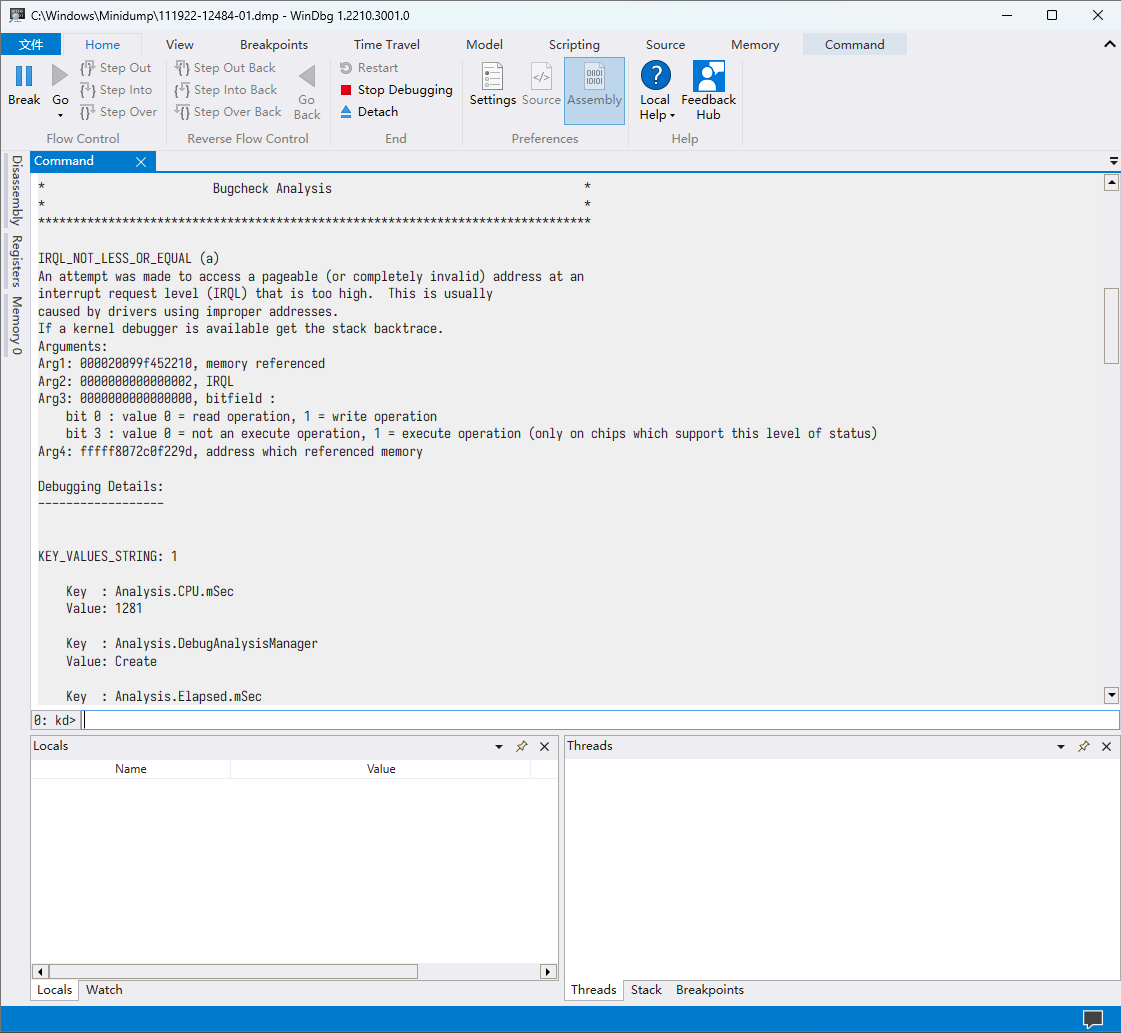
\includegraphics[width=.75\textwidth]{assets/advanced/WinDbg-3.png}
  \caption{WinDbg 的分析结果}
  \label{fig:WinDbg-3}
\end{figure}

但是不要紧张,在里面\cprotect\regcolor{找到以 \MissingVerb{PROCESS_NAME}、\MissingVerb{MODULE_NAME} 与 \MissingVerb{IMAGE_NAME} 开头的几行}。这几行正是与此次蓝屏相关的进程。在这个例子中,这几行分别是

\begin{MissingVerbatim}
PROCESS_NAME:  QQ.exe
MODULE_NAME: nt
IMAGE_NAME:  ntkrnlmp.exe
\end{MissingVerbatim}

此前我们提到过 NT 是如今 Windows 系统内核的名字,查找资料可以发现,这 \MissingVerb{ntkrnlmp.exe} 是系统与硬件交互的程序,看来引起蓝屏的罪魁祸首似乎是 QQ,于是你可以将 QQ 完全卸载重装,然后跟此次蓝屏说再见。

事实上在「分析结果」的那张图片中,程序指出此次蓝屏的蓝屏代码是 \MissingVerb{IRQL_NOT_LESS_OR_EQUAL},若你去网上搜索相关信息的话,看到的大概率是什么「硬件问题」「驱动问题」之类的说法。的确,这种蓝屏与硬件有关,但是什么引起了错误,就只有真正分析才能得到了,这也是为什么需要「对症下药」的缘由。

总结下来,解决蓝屏的一般步骤是:

\begin{enumerate}
  \item 使用 WinDbg 打开最近一次的蓝屏转储文件;
  \item 使用 \MissingVerb{!analyze -v} 命令分析文件;
  \item 找到以 \MissingVerb{PROCESS_NAME}、\MissingVerb{MODULE_NAME} 与 \MissingVerb{IMAGE_NAME} 开头的几行,查看「罪魁祸首」(不熟悉的进程名字可以去网上搜索);
  \item 根据进程情况「对症下药」。
\end{enumerate}

\subsection{设置内存转储方式 *}

\begin{figure}[htb!]
  \centering
  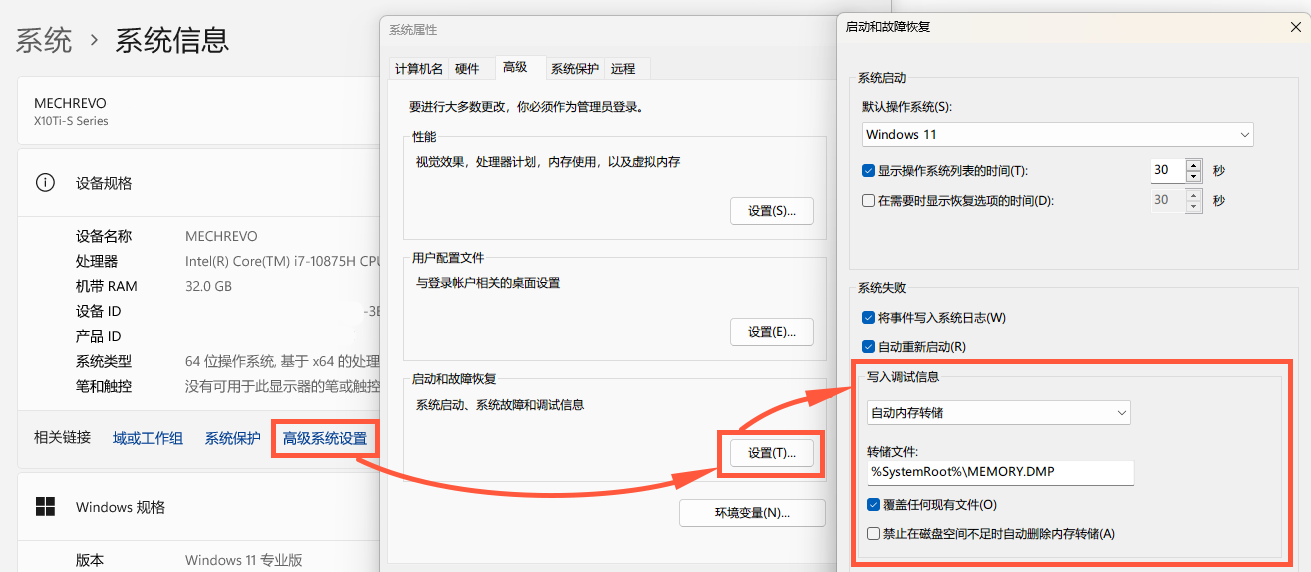
\includegraphics[width=.95\textwidth]{assets/advanced/Dump_Settings.png}
  \caption{设置内存转储}
  \label{fig:Dump_Settings}
\end{figure}

默认情形下,Windows 系统会自动收集内存信息并形成内存转储文件,但你如果发现你的电脑在蓝屏的时候什么也没干,或者想自定义收集选项、查看或设置转储文件的保存位置,那就要前去调整设置。与内存转储相关的设置藏得有点深,找到它的操作步骤是这样的:

\begin{enumerate}
  \item 右击【此电脑】→【属性】来打开「系统信息」页面,你也可以直接按下 \keys{\Windows + Pause} 或 \keys{\Windows + Break} 来打开它;
  \item 点击【高级系统设置】,弹出「系统属性」窗口;
  \item 在「系统属性」窗口中点击【高级】→「启动和故障恢复」下的【设置】,就可以看到「写入调试信息」部分有内存转储的相关设置。
\end{enumerate}

可见,内存转储的类型有五种,除去「小内存转储」默认保存在 \MissingVerb{%SystemRoot%\Minidump} 文件夹下以外,其余选项默认均会生成一个路径为 \MissingVerb{%SystemRoot%\MEMORY.DMP} 的文件。这些路径中的「\MissingVerb」是一个「环境变量」,它指的是电脑上 Windows 系统所在的目录,即 \MissingVerb{C:\Windows}(应该不会有人大动干戈把系统移到别处去吧)。五种内存转储类型的特征大致是这样的:

\begin{itemize}
  \item 小内存转储:大小一般在 256 KB 到几 MB 不等,包含了最基本的崩溃进程、线程、内核堆栈数据与已加载的驱动程序列表,提供最基础的崩溃信息。它的文件名以 \MissingVerb{MMDDYY-NNNNN-XX.dmp} 为格式,\MissingVerb{MMDDYY} 是「月日年」格式的日期,\MissingVerb{XX} 是两位数的当天文件编号。
  \item 核心内存转储:包含崩溃时 Windows 内核、硬件、驱动程序使用的所有内存,但不包含由用户启动的程序所使用的内存。一般而言这些内存已经足够技术人员来确定崩溃的源头了。
  \item 完整内存转储:包含崩溃时 Windows 使用的所有内存。这种转储模式能够收集最完全的信息,但会占用大量空间,要求系统盘中的页面文件要有电脑上所有内存那么大。
  \item 自动内存转储:在页面文件大小由系统自动管理的条件下,系统会自动确保页面文件的大小能尽量完成核心内存转储,当不够用时,页面文件会自动增大并保持大约两星期,之后会恢复原来的大小。
  \item 活动内存转储:类似于「完整内存转储」,但系统自动筛除了与排查主机问题无关的部分,所以通常而言大小会小于完整内存转储,且能提供内存中的绝大部分有用信息。
\end{itemize}

若想修改内存转储文件的存储路径,请为「小内存转储」提供一个文件夹目录,为其他类型提供一个 DMP 文件路径。

\regcolor{默认情形下,Windows 会启用「自动内存转储」},这样能平衡存储空间消耗与崩溃信息收集效率,\regcolor{这也是大多数情形下的推荐选项}。如果\regcolor{存储空间吃紧,建议启用「小内存转储」},让 Windows 至少收集最低限度的崩溃信息。不建议启用「完整内存转储」,它在占用大量空间的同时,收集信息的收益并没有比「核心内存转储」高出多少。「活动内存转储」适用于大量运行虚拟机时的情形,它会筛去虚拟机使用的内存,只关注物理主机。

\section{微软教你「搞定」蓝屏}

\begin{warning}
  不推荐使用本节的方法排查错误,此处只是为了展示「遵从提示」的情况。
\end{warning}

再次审视\autoref{fig:Win-11-BSoD} 的 Windows 10/11 的蓝屏界面,这上面说
\begin{quoting}
  有关此问题的详细信息和可能的解决办法,请访问
  
  \url{https://www.windows.com/stopcode}
\end{quoting}

好咯,那我们就去看看。用手机扫码或在电脑上手动访问这个页面,映入眼帘的是如\autoref{fig:Stopcode-Webpage} 这样的说明。

\begin{figure}[htb!]
  \centering
  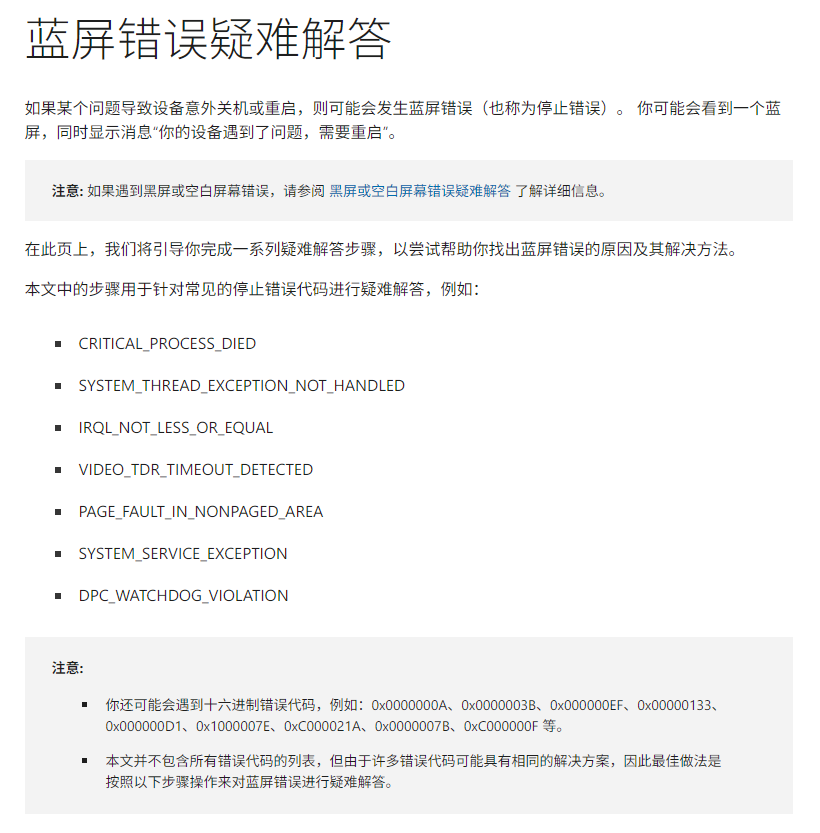
\includegraphics[width=.65\textwidth]{assets/advanced/Stopcode-Webpage.png}
  \caption{二维码指向的网页}
  \label{fig:Stopcode-Webpage}
\end{figure}

嗯……它说:

\begin{quoting}
  本文并不包含所有错误代码的列表,但由于许多错误代码可能具有相同的解决方案,因此最佳做法是按照以下步骤操作来对蓝屏错误进行疑难解答。
\end{quoting}

翻译一下就是:我们估计以下方案可能能够搞定蓝屏,推荐你试试,但搞不定我们也没办法。

再往下翻,根据提示行事,你会发现微软列出的解决方案包括「卸载第三方软件」「回退、禁用或卸载驱动程序」「移除外接硬件」等,事实上……也没错,解决蓝屏确实要除掉点什么东西,但问题在于这「解决方案」只告诉我们类似「如何卸载软件」的方法论,却不告诉我们「应该卸载什么软件」之类的具体措施。归根结底还是造成蓝屏的原因千变万化,不能简单一概而论。所以微软也在教你如何「碰运气」……不愧是你,微软。

\practice

\begin{enumerate}
  \item 你还见过什么样类似「蓝屏」性质的系统错误界面,它们与「蓝屏」有何异同?
  \item 尝试自己分析一个蓝屏转储文件,如果自己电脑里没有可以找找朋友的电脑,或者前往网页版的这一题用我们提供的文件练练手。
\end{enumerate}